\section{Software Design}
    In this section, overall design of the project is discussed, presenting arguments for various choices made and the outcomes of such choices. Existing and possible dependencies, constraints or limitations are mentioned here.
    
    In \cref{architecture} a project's architecture overview is given, showing the structure of various components at play, along with the intention and reasoning behind it.
    
    The \cref{techstack} presents various technologies chosen to develop the software and fulfil the requirements specified in previous chapters.
    
    Lastly, \cref{assumptionsdependencies} discusses how current design impacts the software's dependencies, installation and running process, and existing constraints.
    
    \subsection{Project's Architecture} \label{architecture}
    
        First of all, the project structure is presented here. The project is structured in a way that in future it could be extended into micro services architecture model, where each component can be easily customised, combined with others, added or taken away based on needs. In this case, there are three components: Textual Entailment, Twitter Mining and Argumentation Framework. All of them connect to a central point from where the application is initiated.
        
        \begin{figure}[!htbp]
            \centering
            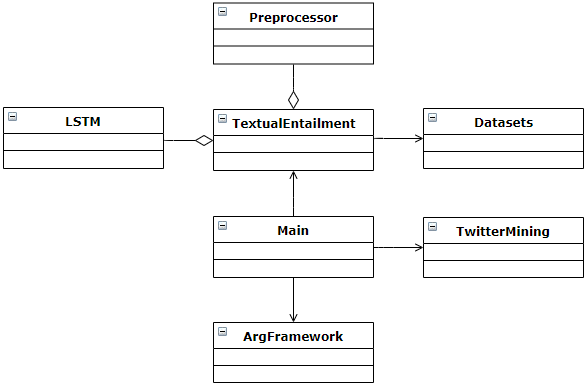
\includegraphics[scale=0.75]{img/classdiag.png}
            \caption{Class Diagram}
            \label{fig:classdiag}
        \end{figure}
        
        The figure above does not list class methods or fields because they are extensively discussed in implementation chapter alongside code listings. Textual Entailment class is responsible for coordinating everything related to deep neural networks and textual entailment itself. Datasets class checks whether the data is present in a folder and if not, is downloaded and unzipped. Preprocessor is responsible for reading downloaded data, transforming it into sequences of numbers and the result of that is passed to LSTM class by Textual Entailment for neural network setup. LSTM, as mentioned, is responsible for managing neural networks. TwitterMining, on the other hand, used for gathering tweets and at the same time cleaning the textual data, preparing for analysis. ArgFramework is a class that is tasked with creating argument frameworks, drawing them and providing methods to conduct analysis on the graphs.
        
        This breakdown of software functions provides the needed flexibility to later on expand into micro services model, hosting each process on a cloud server, that is customised to that service's hardware needs and can be accessed platform independently via the use of \gls{api}.
        
        A popular alternative is to build a monolithic application, where all processes are bundled together in a single application. The benefits of this involve centralised code base, more tightly managed code and in some cases better understanding of various dependencies and interrelationships between different classes or parts of software. Also, an argument could be made that this is a more cost efficient solution as only a single machine is required. 
        
        In contrast, not all components are equal. At this moment, the Textual Entailment part requires way more hardware resources to operate, than, for example, Twitter mining functions. Especially when talking about scalability and addition of other angles of analysis (e.g. bipolar versus abstract argument frameworks) or sources to gather textual data (e.g. Facebook, Wikipedia, news sites), or even argument relation prediction techniques (e.g. logistic regression among others), the choice of separating each part becomes a much more natural solution, that can also simplify a lot of development work.
    
    \subsection{Technology Stack} \label{techstack}
        Technological choices are presented and explained here in detail. Alternatives are also discussed and argued for and against. This section covers the discussions of Programming Languages, Dependency and Package Managers, and Programming Libraries.
        
        \subsubsection{Programming Language}
            Programming language Python version 3.7. There is a reason why Python is the de facto language for all purposes Machine Learning, Deep Learning, Data Science and Analysis, and this is because of the vast amount of libraries that enable the developer to easily incorporate the functionality in any project. Nonetheless, the core calculations of those libraries are done in C/C++ language and Python is used as a wrapper for easy access and compatibility, which makes memory intensive computations all the more efficient. 
            
            Even though C/C++ offers much more flexibility in terms of memory management and performance optimisation, the core data science and machine learning libraries and frameworks, for historical reasons, are mostly saturated in Python language, while C/C++ is left as more of a pure hardware and game development language. Additionally, Python requires less code and its' syntax is less strict, which is probably why it is a popular language among research communities, allowing for faster prototyping of new algorithms and ideas.
            
            Older version of Python2.7 is still a popular alternative. Currently, most of the frameworks and libraries are still supporting this version of Python, as well as there are older frameworks that have not yet updated to be compatible with version 3.7 and are only available on 2.7. But with Python2.7 being quite old in technology terms and some framework developers announcing that in a couple of years they will not be supporting Python2.7 anymore makes this a less attractive option. There are also syntactical differences between versions, with Python3.7 offering a more cleaner and concise coding options. Overall, Python2.7 is supported today only because of backward compatibility reasons and not because it is being developed or updated independently by the language creators.
        
        \subsubsection{Dependency and Package Managers}
            Anaconda was used as a package and dependency manager for Python, allowing easy and quick addition of various external libraries (Tweepy, TensorFlow and various sub dependencies). Moreover, PyCharm was used to fulfil the role of Integrated Development Environment for Python, mostly because of it having a lot more features than the free counterparts, as students can get Ultimate license free of charge for a year. Alternatively, Python has PIP which is also a package manager, albeit more lightweight in that it is purely a command line interface. Anaconda comes with a graphical interface and a prepackaged bundle of most common libraries, which are not included if PIP was chosen as default package manager.
            
        \subsubsection{Twitter Data Access Library}
            Tweepy was chosen to be used as Twitter API access library, because, first of all, is one of the not many libraries that are still maintained and updated today, constantly providing more and more flexibility with gathering of Twitter Data, and secondly, because of documentation providing lots of examples how to quickly set up and get up to speed. An alternative could have been to create a custom \gls{api} to access twitter posts. This would have led to more flexibility from development point of view, but increased time spend developing it is not worth it as existing solution proves sufficient for the task at hand.
            
        \subsubsection{Deep Neural Network Development Library Framework}
            The most popular library that delivers upon the objectives of the project is TensorFlow, and as such it is used in this project. Its' popularity speaks volumes as there is a vast amount of guides easily accessible and extendable into solving complex problems (such as Recognizing Textual Entailment, for example). Also, the documentation is full with up to date details and examples clearly explaining differences between previous and future (yet to be released) versions. Another popular library is PyTorch, it also features a lot of functions that can perform the same tasks as TensorFlow. Difference being that PyTorch is a newer framework, naturally meaning smaller community and lesser flexibility (at least until it has fully caught up to the existing TensorFlow framework), but it is offering new ways of doing things (in some functions) which may prove useful in some cases. The verdict is that currently, TensorFlow offers higher control of parameter tuning for the purpose of training and developing \gls{lstm} networks.
            
        \subsubsection{Argumentation Framework Construction Library}
            To draw the graph network and be able to properly analyse it, a special library is required. One such library is NetworkX, which is mainly used to analyse networks in the traditional sense, providing different implementations of popular analysis algorithms, such as topological sort, breadth and depth first searches, Dijkstra's algorithm and so on. This library is not a new one and has existed for a while, which also makes this a positive as a lot of information is available online on different forums and discussion boards. Since argumentation frameworks are essentially network graphs (both are represented with vertices and directional edges between them), this library is a perfect choice for the matter. In Python world, there are not many alternatives. Most other graph network libraries that are popular are coded for C/C++ environments, because research and analysis of networks is computationally challenging task and the performance management that C/C++ provide is beneficial. Unfortunately, this project cannot make use of those benefits because it is developed in Python, for main reason being that it is more focused towards the Machine Learning/Artificial Intelligence side of things than pure graph research.
        
    \subsection{Assumptions, Dependencies and Constraints} \label{assumptionsdependencies}
        This section explains the technical dependencies required to run the project in its' current state.
        
        The project is open source, this means that in order to install it and therefore run it, the user has to manually make sure that all dependencies are set up. This requires knowledge of command line interfaces, having python installed, integrated development environment (of choice) is recommended but not required.
        
        While this is an inconvenience for people who are not technically literate, the intended audience for the project are users that are comfortable with reading python code and can customise it to suit their research needs. This includes training different models, tuning parameters and adding new argumentation framework analysis avenues via open source contribution.
        
        All of this could have been done the other way around, constructing a single analysis model and specific criteria using which the argument framework is evaluated. While this would undoubtedly make the program more user friendly and possibly even a marketable product, that is not the intended result of the project. One of project aims listed previously is contributing to artificial intelligence research community, and the best way this can be done is via open source code providing a starting point and hopefully bring about necessary breakthrough that advances this specific subfield of argument mining and analysis.

        Everything in the project is controlled via command line interface. This means that running the software and user getting informed of different stages that software enters, including results, is presented in text format. A proper graphical interface is to be considered in future, as user experience is not the focus of the project currently.
        
        Additionally, the Twitter \gls{api} has some limitations of its' own. First of all, the data is handicapped to a specific rate that the user can access the \gls{api} in a short amount of time. Twitter does this to shield itself from abuse and potential \gls{ddos} attacks. Secondly, the only data that is accessible via Twitter \gls{api} is not older than 7 days and has to be at least 1 hour old. The main complication here is that if the user wants to analyse a topic that was hotly debated and argued previously (as in, older than 7 days), this poses a problem. The only solution is to monitor current affairs on Twitter and data mine tweets in advance, or as things are happening, and save them for later use or analysis.